% Created by tikzDevice version 0.10.1 on 2016-07-18 19:10:51
% !TEX encoding = UTF-8 Unicode
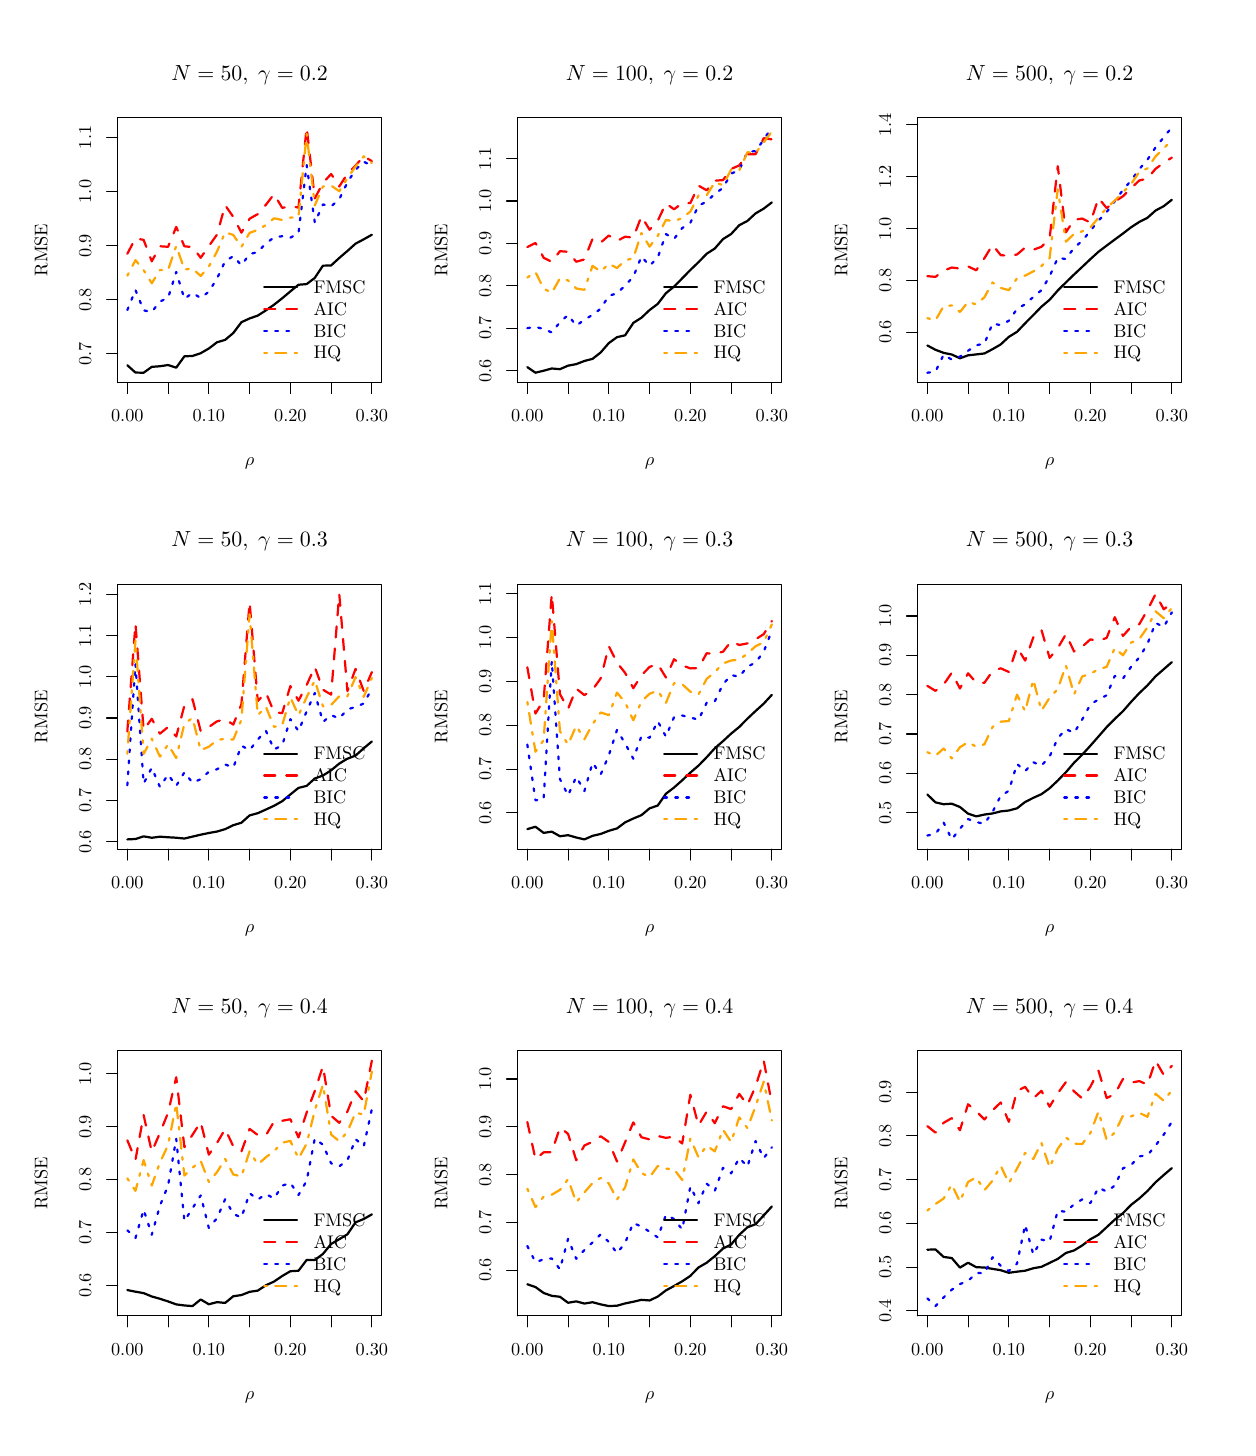
\begin{tikzpicture}[x=1pt,y=1pt]
\definecolor{fillColor}{RGB}{255,255,255}
\path[use as bounding box,fill=fillColor,fill opacity=0.00] (0,0) rectangle (433.62,505.89);
\begin{scope}
\path[clip] ( 32.47,377.65) rectangle (127.91,473.42);
\definecolor{drawColor}{RGB}{0,0,0}

\path[draw=drawColor,line width= 0.8pt,line join=round,line cap=round] ( 36.01,383.90) --
	( 38.95,381.26) --
	( 41.90,381.20) --
	( 44.84,383.32) --
	( 47.79,383.54) --
	( 50.73,383.98) --
	( 53.68,383.03) --
	( 56.63,387.12) --
	( 59.57,387.26) --
	( 62.52,388.26) --
	( 65.46,389.95) --
	( 68.41,392.20) --
	( 71.35,393.07) --
	( 74.30,395.55) --
	( 77.24,399.46) --
	( 80.19,400.81) --
	( 83.14,401.85) --
	( 86.08,403.72) --
	( 89.03,405.78) --
	( 91.97,408.10) --
	( 94.92,410.59) --
	( 97.86,412.99) --
	(100.81,413.23) --
	(103.75,415.46) --
	(106.70,419.88) --
	(109.65,419.97) --
	(112.59,422.67) --
	(115.54,425.20) --
	(118.48,427.84) --
	(121.43,429.40) --
	(124.37,431.06);
\end{scope}
\begin{scope}
\path[clip] (  0.00,  0.00) rectangle (433.62,505.89);
\definecolor{drawColor}{RGB}{0,0,0}

\path[draw=drawColor,line width= 0.4pt,line join=round,line cap=round] ( 36.01,377.65) -- (124.37,377.65);

\path[draw=drawColor,line width= 0.4pt,line join=round,line cap=round] ( 36.01,377.65) -- ( 36.01,373.69);

\path[draw=drawColor,line width= 0.4pt,line join=round,line cap=round] ( 50.73,377.65) -- ( 50.73,373.69);

\path[draw=drawColor,line width= 0.4pt,line join=round,line cap=round] ( 65.46,377.65) -- ( 65.46,373.69);

\path[draw=drawColor,line width= 0.4pt,line join=round,line cap=round] ( 80.19,377.65) -- ( 80.19,373.69);

\path[draw=drawColor,line width= 0.4pt,line join=round,line cap=round] ( 94.92,377.65) -- ( 94.92,373.69);

\path[draw=drawColor,line width= 0.4pt,line join=round,line cap=round] (109.65,377.65) -- (109.65,373.69);

\path[draw=drawColor,line width= 0.4pt,line join=round,line cap=round] (124.37,377.65) -- (124.37,373.69);

\node[text=drawColor,anchor=base,inner sep=0pt, outer sep=0pt, scale=  0.66] at ( 36.01,363.40) {0.00};

\node[text=drawColor,anchor=base,inner sep=0pt, outer sep=0pt, scale=  0.66] at ( 65.46,363.40) {0.10};

\node[text=drawColor,anchor=base,inner sep=0pt, outer sep=0pt, scale=  0.66] at ( 94.92,363.40) {0.20};

\node[text=drawColor,anchor=base,inner sep=0pt, outer sep=0pt, scale=  0.66] at (124.37,363.40) {0.30};

\path[draw=drawColor,line width= 0.4pt,line join=round,line cap=round] ( 32.47,388.00) -- ( 32.47,466.24);

\path[draw=drawColor,line width= 0.4pt,line join=round,line cap=round] ( 32.47,388.00) -- ( 28.51,388.00);

\path[draw=drawColor,line width= 0.4pt,line join=round,line cap=round] ( 32.47,407.56) -- ( 28.51,407.56);

\path[draw=drawColor,line width= 0.4pt,line join=round,line cap=round] ( 32.47,427.12) -- ( 28.51,427.12);

\path[draw=drawColor,line width= 0.4pt,line join=round,line cap=round] ( 32.47,446.68) -- ( 28.51,446.68);

\path[draw=drawColor,line width= 0.4pt,line join=round,line cap=round] ( 32.47,466.24) -- ( 28.51,466.24);

\node[text=drawColor,rotate= 90.00,anchor=base,inner sep=0pt, outer sep=0pt, scale=  0.66] at ( 22.97,388.00) {0.7};

\node[text=drawColor,rotate= 90.00,anchor=base,inner sep=0pt, outer sep=0pt, scale=  0.66] at ( 22.97,407.56) {0.8};

\node[text=drawColor,rotate= 90.00,anchor=base,inner sep=0pt, outer sep=0pt, scale=  0.66] at ( 22.97,427.12) {0.9};

\node[text=drawColor,rotate= 90.00,anchor=base,inner sep=0pt, outer sep=0pt, scale=  0.66] at ( 22.97,446.68) {1.0};

\node[text=drawColor,rotate= 90.00,anchor=base,inner sep=0pt, outer sep=0pt, scale=  0.66] at ( 22.97,466.24) {1.1};

\path[draw=drawColor,line width= 0.4pt,line join=round,line cap=round] ( 32.47,377.65) --
	(127.91,377.65) --
	(127.91,473.42) --
	( 32.47,473.42) --
	( 32.47,377.65);
\end{scope}
\begin{scope}
\path[clip] (  0.00,337.26) rectangle (144.54,505.89);
\definecolor{drawColor}{RGB}{0,0,0}

\node[text=drawColor,anchor=base,inner sep=0pt, outer sep=0pt, scale=  0.79] at ( 80.19,486.92) {\bfseries $N=50, \;\gamma=0.2$};

\node[text=drawColor,anchor=base,inner sep=0pt, outer sep=0pt, scale=  0.66] at ( 80.19,347.56) {$\rho$};

\node[text=drawColor,rotate= 90.00,anchor=base,inner sep=0pt, outer sep=0pt, scale=  0.66] at (  7.13,425.53) {RMSE};
\end{scope}
\begin{scope}
\path[clip] ( 32.47,377.65) rectangle (127.91,473.42);
\definecolor{drawColor}{RGB}{255,0,0}

\path[draw=drawColor,line width= 0.8pt,dash pattern=on 4pt off 4pt ,line join=round,line cap=round] ( 36.01,424.18) --
	( 38.95,429.77) --
	( 41.90,429.20) --
	( 44.84,421.45) --
	( 47.79,426.90) --
	( 50.73,426.70) --
	( 53.68,433.89) --
	( 56.63,426.88) --
	( 59.57,426.61) --
	( 62.52,422.74) --
	( 65.46,426.95) --
	( 68.41,431.10) --
	( 71.35,441.72) --
	( 74.30,437.51) --
	( 77.24,431.80) --
	( 80.19,436.85) --
	( 83.14,438.52) --
	( 86.08,441.88) --
	( 89.03,445.74) --
	( 91.97,440.78) --
	( 94.92,441.37) --
	( 97.86,440.88) --
	(100.81,469.87) --
	(103.75,444.20) --
	(106.70,449.78) --
	(109.65,453.03) --
	(112.59,448.49) --
	(115.54,453.11) --
	(118.48,456.06) --
	(121.43,459.42) --
	(124.37,457.67);
\definecolor{drawColor}{RGB}{0,0,255}

\path[draw=drawColor,line width= 0.8pt,dash pattern=on 1pt off 3pt ,line join=round,line cap=round] ( 36.01,403.85) --
	( 38.95,411.09) --
	( 41.90,403.74) --
	( 44.84,403.15) --
	( 47.79,406.94) --
	( 50.73,408.23) --
	( 53.68,417.61) --
	( 56.63,407.90) --
	( 59.57,410.05) --
	( 62.52,408.18) --
	( 65.46,410.49) --
	( 68.41,415.21) --
	( 71.35,421.50) --
	( 74.30,423.30) --
	( 77.24,420.02) --
	( 80.19,424.09) --
	( 83.14,424.77) --
	( 86.08,427.99) --
	( 89.03,430.05) --
	( 91.97,430.54) --
	( 94.92,430.01) --
	( 97.86,431.59) --
	(100.81,456.25) --
	(103.75,435.43) --
	(106.70,442.00) --
	(109.65,441.32) --
	(112.59,443.86) --
	(115.54,450.01) --
	(118.48,454.53) --
	(121.43,457.46) --
	(124.37,456.02);
\definecolor{drawColor}{RGB}{255,165,0}

\path[draw=drawColor,line width= 0.8pt,dash pattern=on 1pt off 3pt on 4pt off 3pt ,line join=round,line cap=round] ( 36.01,416.27) --
	( 38.95,421.87) --
	( 41.90,418.27) --
	( 44.84,413.52) --
	( 47.79,418.30) --
	( 50.73,418.29) --
	( 53.68,427.03) --
	( 56.63,418.49) --
	( 59.57,418.85) --
	( 62.52,416.15) --
	( 65.46,419.55) --
	( 68.41,424.98) --
	( 71.35,431.97) --
	( 74.30,430.96) --
	( 77.24,426.70) --
	( 80.19,431.74) --
	( 83.14,432.81) --
	( 86.08,434.56) --
	( 89.03,437.00) --
	( 91.97,436.41) --
	( 94.92,437.24) --
	( 97.86,437.55) --
	(100.81,467.50) --
	(103.75,441.70) --
	(106.70,448.50) --
	(109.65,448.82) --
	(112.59,446.79) --
	(115.54,451.50) --
	(118.48,455.71) --
	(121.43,459.40) --
	(124.37,456.98);
\definecolor{drawColor}{RGB}{0,0,0}

\path[draw=drawColor,line width= 0.8pt,line join=round,line cap=round] ( 85.47,412.20) -- ( 97.35,412.20);
\definecolor{drawColor}{RGB}{255,0,0}

\path[draw=drawColor,line width= 0.8pt,dash pattern=on 4pt off 4pt ,line join=round,line cap=round] ( 85.47,404.28) -- ( 97.35,404.28);
\definecolor{drawColor}{RGB}{0,0,255}

\path[draw=drawColor,line width= 0.8pt,dash pattern=on 1pt off 3pt ,line join=round,line cap=round] ( 85.47,396.36) -- ( 97.35,396.36);
\definecolor{drawColor}{RGB}{255,165,0}

\path[draw=drawColor,line width= 0.8pt,dash pattern=on 1pt off 3pt on 4pt off 3pt ,line join=round,line cap=round] ( 85.47,388.44) -- ( 97.35,388.44);
\definecolor{drawColor}{RGB}{0,0,0}

\node[text=drawColor,anchor=base west,inner sep=0pt, outer sep=0pt, scale=  0.66] at (103.29,409.93) {FMSC};

\node[text=drawColor,anchor=base west,inner sep=0pt, outer sep=0pt, scale=  0.66] at (103.29,402.01) {AIC};

\node[text=drawColor,anchor=base west,inner sep=0pt, outer sep=0pt, scale=  0.66] at (103.29,394.09) {BIC};

\node[text=drawColor,anchor=base west,inner sep=0pt, outer sep=0pt, scale=  0.66] at (103.29,386.17) {HQ};
\end{scope}
\begin{scope}
\path[clip] (177.01,377.65) rectangle (272.45,473.42);
\definecolor{drawColor}{RGB}{0,0,0}

\path[draw=drawColor,line width= 0.8pt,line join=round,line cap=round] (180.55,383.22) --
	(183.49,381.20) --
	(186.44,381.93) --
	(189.38,382.73) --
	(192.33,382.48) --
	(195.27,383.76) --
	(198.22,384.30) --
	(201.17,385.45) --
	(204.11,386.21) --
	(207.06,388.53) --
	(210.00,391.92) --
	(212.95,394.04) --
	(215.89,394.72) --
	(218.84,399.20) --
	(221.78,401.07) --
	(224.73,403.86) --
	(227.68,406.07) --
	(230.62,409.93) --
	(233.57,412.33) --
	(236.51,415.30) --
	(239.46,418.33) --
	(242.40,421.14) --
	(245.35,424.19) --
	(248.29,426.08) --
	(251.24,429.47) --
	(254.19,431.32) --
	(257.13,434.51) --
	(260.08,436.05) --
	(263.02,438.77) --
	(265.97,440.49) --
	(268.91,442.76);
\end{scope}
\begin{scope}
\path[clip] (  0.00,  0.00) rectangle (433.62,505.89);
\definecolor{drawColor}{RGB}{0,0,0}

\path[draw=drawColor,line width= 0.4pt,line join=round,line cap=round] (180.55,377.65) -- (268.91,377.65);

\path[draw=drawColor,line width= 0.4pt,line join=round,line cap=round] (180.55,377.65) -- (180.55,373.69);

\path[draw=drawColor,line width= 0.4pt,line join=round,line cap=round] (195.27,377.65) -- (195.27,373.69);

\path[draw=drawColor,line width= 0.4pt,line join=round,line cap=round] (210.00,377.65) -- (210.00,373.69);

\path[draw=drawColor,line width= 0.4pt,line join=round,line cap=round] (224.73,377.65) -- (224.73,373.69);

\path[draw=drawColor,line width= 0.4pt,line join=round,line cap=round] (239.46,377.65) -- (239.46,373.69);

\path[draw=drawColor,line width= 0.4pt,line join=round,line cap=round] (254.19,377.65) -- (254.19,373.69);

\path[draw=drawColor,line width= 0.4pt,line join=round,line cap=round] (268.91,377.65) -- (268.91,373.69);

\node[text=drawColor,anchor=base,inner sep=0pt, outer sep=0pt, scale=  0.66] at (180.55,363.40) {0.00};

\node[text=drawColor,anchor=base,inner sep=0pt, outer sep=0pt, scale=  0.66] at (210.00,363.40) {0.10};

\node[text=drawColor,anchor=base,inner sep=0pt, outer sep=0pt, scale=  0.66] at (239.46,363.40) {0.20};

\node[text=drawColor,anchor=base,inner sep=0pt, outer sep=0pt, scale=  0.66] at (268.91,363.40) {0.30};

\path[draw=drawColor,line width= 0.4pt,line join=round,line cap=round] (177.01,381.99) -- (177.01,458.56);

\path[draw=drawColor,line width= 0.4pt,line join=round,line cap=round] (177.01,381.99) -- (173.05,381.99);

\path[draw=drawColor,line width= 0.4pt,line join=round,line cap=round] (177.01,397.30) -- (173.05,397.30);

\path[draw=drawColor,line width= 0.4pt,line join=round,line cap=round] (177.01,412.62) -- (173.05,412.62);

\path[draw=drawColor,line width= 0.4pt,line join=round,line cap=round] (177.01,427.93) -- (173.05,427.93);

\path[draw=drawColor,line width= 0.4pt,line join=round,line cap=round] (177.01,443.25) -- (173.05,443.25);

\path[draw=drawColor,line width= 0.4pt,line join=round,line cap=round] (177.01,458.56) -- (173.05,458.56);

\node[text=drawColor,rotate= 90.00,anchor=base,inner sep=0pt, outer sep=0pt, scale=  0.66] at (167.51,381.99) {0.6};

\node[text=drawColor,rotate= 90.00,anchor=base,inner sep=0pt, outer sep=0pt, scale=  0.66] at (167.51,397.30) {0.7};

\node[text=drawColor,rotate= 90.00,anchor=base,inner sep=0pt, outer sep=0pt, scale=  0.66] at (167.51,412.62) {0.8};

\node[text=drawColor,rotate= 90.00,anchor=base,inner sep=0pt, outer sep=0pt, scale=  0.66] at (167.51,427.93) {0.9};

\node[text=drawColor,rotate= 90.00,anchor=base,inner sep=0pt, outer sep=0pt, scale=  0.66] at (167.51,443.25) {1.0};

\node[text=drawColor,rotate= 90.00,anchor=base,inner sep=0pt, outer sep=0pt, scale=  0.66] at (167.51,458.56) {1.1};

\path[draw=drawColor,line width= 0.4pt,line join=round,line cap=round] (177.01,377.65) --
	(272.45,377.65) --
	(272.45,473.42) --
	(177.01,473.42) --
	(177.01,377.65);
\end{scope}
\begin{scope}
\path[clip] (144.54,337.26) rectangle (289.08,505.89);
\definecolor{drawColor}{RGB}{0,0,0}

\node[text=drawColor,anchor=base,inner sep=0pt, outer sep=0pt, scale=  0.79] at (224.73,486.92) {\bfseries $N=100, \;\gamma=0.2$};

\node[text=drawColor,anchor=base,inner sep=0pt, outer sep=0pt, scale=  0.66] at (224.73,347.56) {$\rho$};

\node[text=drawColor,rotate= 90.00,anchor=base,inner sep=0pt, outer sep=0pt, scale=  0.66] at (151.67,425.53) {RMSE};
\end{scope}
\begin{scope}
\path[clip] (177.01,377.65) rectangle (272.45,473.42);
\definecolor{drawColor}{RGB}{255,0,0}

\path[draw=drawColor,line width= 0.8pt,dash pattern=on 4pt off 4pt ,line join=round,line cap=round] (180.55,426.60) --
	(183.49,428.10) --
	(186.44,422.76) --
	(189.38,421.25) --
	(192.33,425.13) --
	(195.27,424.89) --
	(198.22,421.31) --
	(201.17,422.14) --
	(204.11,429.57) --
	(207.06,428.22) --
	(210.00,430.78) --
	(212.95,428.79) --
	(215.89,430.36) --
	(218.84,430.00) --
	(221.78,437.73) --
	(224.73,432.88) --
	(227.68,436.12) --
	(230.62,442.36) --
	(233.57,440.26) --
	(236.51,442.48) --
	(239.46,442.51) --
	(242.40,448.81) --
	(245.35,447.12) --
	(248.29,450.60) --
	(251.24,450.80) --
	(254.19,454.83) --
	(257.13,456.12) --
	(260.08,460.11) --
	(263.02,460.16) --
	(265.97,465.94) --
	(268.91,465.51);
\definecolor{drawColor}{RGB}{0,0,255}

\path[draw=drawColor,line width= 0.8pt,dash pattern=on 1pt off 3pt ,line join=round,line cap=round] (180.55,397.32) --
	(183.49,397.71) --
	(186.44,397.06) --
	(189.38,395.74) --
	(192.33,399.47) --
	(195.27,402.07) --
	(198.22,398.22) --
	(201.17,400.33) --
	(204.11,402.11) --
	(207.06,404.33) --
	(210.00,409.04) --
	(212.95,409.85) --
	(215.89,412.72) --
	(218.84,415.83) --
	(221.78,423.21) --
	(224.73,419.85) --
	(227.68,422.81) --
	(230.62,431.31) --
	(233.57,429.55) --
	(236.51,433.47) --
	(239.46,435.38) --
	(242.40,441.57) --
	(245.35,443.05) --
	(248.29,445.82) --
	(251.24,447.99) --
	(254.19,453.16) --
	(257.13,454.38) --
	(260.08,461.06) --
	(263.02,461.25) --
	(265.97,465.44) --
	(268.91,469.87);
\definecolor{drawColor}{RGB}{255,165,0}

\path[draw=drawColor,line width= 0.8pt,dash pattern=on 1pt off 3pt on 4pt off 3pt ,line join=round,line cap=round] (180.55,415.59) --
	(183.49,417.56) --
	(186.44,411.60) --
	(189.38,410.05) --
	(192.33,415.30) --
	(195.27,414.55) --
	(198.22,411.64) --
	(201.17,411.16) --
	(204.11,419.82) --
	(207.06,417.72) --
	(210.00,420.58) --
	(212.95,419.03) --
	(215.89,421.79) --
	(218.84,422.58) --
	(221.78,431.67) --
	(224.73,426.75) --
	(227.68,430.69) --
	(230.62,436.38) --
	(233.57,435.95) --
	(236.51,437.12) --
	(239.46,439.44) --
	(242.40,445.22) --
	(245.35,445.33) --
	(248.29,450.01) --
	(251.24,448.97) --
	(254.19,454.56) --
	(257.13,454.30) --
	(260.08,460.89) --
	(263.02,460.59) --
	(265.97,464.44) --
	(268.91,468.34);
\definecolor{drawColor}{RGB}{0,0,0}

\path[draw=drawColor,line width= 0.8pt,line join=round,line cap=round] (230.01,412.20) -- (241.89,412.20);
\definecolor{drawColor}{RGB}{255,0,0}

\path[draw=drawColor,line width= 0.8pt,dash pattern=on 4pt off 4pt ,line join=round,line cap=round] (230.01,404.28) -- (241.89,404.28);
\definecolor{drawColor}{RGB}{0,0,255}

\path[draw=drawColor,line width= 0.8pt,dash pattern=on 1pt off 3pt ,line join=round,line cap=round] (230.01,396.36) -- (241.89,396.36);
\definecolor{drawColor}{RGB}{255,165,0}

\path[draw=drawColor,line width= 0.8pt,dash pattern=on 1pt off 3pt on 4pt off 3pt ,line join=round,line cap=round] (230.01,388.44) -- (241.89,388.44);
\definecolor{drawColor}{RGB}{0,0,0}

\node[text=drawColor,anchor=base west,inner sep=0pt, outer sep=0pt, scale=  0.66] at (247.83,409.93) {FMSC};

\node[text=drawColor,anchor=base west,inner sep=0pt, outer sep=0pt, scale=  0.66] at (247.83,402.01) {AIC};

\node[text=drawColor,anchor=base west,inner sep=0pt, outer sep=0pt, scale=  0.66] at (247.83,394.09) {BIC};

\node[text=drawColor,anchor=base west,inner sep=0pt, outer sep=0pt, scale=  0.66] at (247.83,386.17) {HQ};
\end{scope}
\begin{scope}
\path[clip] (321.55,377.65) rectangle (416.99,473.42);
\definecolor{drawColor}{RGB}{0,0,0}

\path[draw=drawColor,line width= 0.8pt,line join=round,line cap=round] (325.09,391.05) --
	(328.03,389.49) --
	(330.98,388.38) --
	(333.92,387.78) --
	(336.87,386.42) --
	(339.81,387.48) --
	(342.76,387.82) --
	(345.71,388.16) --
	(348.65,389.71) --
	(351.60,391.43) --
	(354.54,394.16) --
	(357.49,395.97) --
	(360.43,399.06) --
	(363.38,402.03) --
	(366.32,405.06) --
	(369.27,407.55) --
	(372.22,410.91) --
	(375.16,413.83) --
	(378.11,416.69) --
	(381.05,419.44) --
	(384.00,422.23) --
	(386.94,424.91) --
	(389.89,427.14) --
	(392.83,429.33) --
	(395.78,431.50) --
	(398.73,433.77) --
	(401.67,435.68) --
	(404.62,437.18) --
	(407.56,439.81) --
	(410.51,441.38) --
	(413.45,443.70);
\end{scope}
\begin{scope}
\path[clip] (  0.00,  0.00) rectangle (433.62,505.89);
\definecolor{drawColor}{RGB}{0,0,0}

\path[draw=drawColor,line width= 0.4pt,line join=round,line cap=round] (325.09,377.65) -- (413.45,377.65);

\path[draw=drawColor,line width= 0.4pt,line join=round,line cap=round] (325.09,377.65) -- (325.09,373.69);

\path[draw=drawColor,line width= 0.4pt,line join=round,line cap=round] (339.81,377.65) -- (339.81,373.69);

\path[draw=drawColor,line width= 0.4pt,line join=round,line cap=round] (354.54,377.65) -- (354.54,373.69);

\path[draw=drawColor,line width= 0.4pt,line join=round,line cap=round] (369.27,377.65) -- (369.27,373.69);

\path[draw=drawColor,line width= 0.4pt,line join=round,line cap=round] (384.00,377.65) -- (384.00,373.69);

\path[draw=drawColor,line width= 0.4pt,line join=round,line cap=round] (398.73,377.65) -- (398.73,373.69);

\path[draw=drawColor,line width= 0.4pt,line join=round,line cap=round] (413.45,377.65) -- (413.45,373.69);

\node[text=drawColor,anchor=base,inner sep=0pt, outer sep=0pt, scale=  0.66] at (325.09,363.40) {0.00};

\node[text=drawColor,anchor=base,inner sep=0pt, outer sep=0pt, scale=  0.66] at (354.54,363.40) {0.10};

\node[text=drawColor,anchor=base,inner sep=0pt, outer sep=0pt, scale=  0.66] at (384.00,363.40) {0.20};

\node[text=drawColor,anchor=base,inner sep=0pt, outer sep=0pt, scale=  0.66] at (413.45,363.40) {0.30};

\path[draw=drawColor,line width= 0.4pt,line join=round,line cap=round] (321.55,395.84) -- (321.55,470.76);

\path[draw=drawColor,line width= 0.4pt,line join=round,line cap=round] (321.55,395.84) -- (317.59,395.84);

\path[draw=drawColor,line width= 0.4pt,line join=round,line cap=round] (321.55,414.57) -- (317.59,414.57);

\path[draw=drawColor,line width= 0.4pt,line join=round,line cap=round] (321.55,433.30) -- (317.59,433.30);

\path[draw=drawColor,line width= 0.4pt,line join=round,line cap=round] (321.55,452.03) -- (317.59,452.03);

\path[draw=drawColor,line width= 0.4pt,line join=round,line cap=round] (321.55,470.76) -- (317.59,470.76);

\node[text=drawColor,rotate= 90.00,anchor=base,inner sep=0pt, outer sep=0pt, scale=  0.66] at (312.05,395.84) {0.6};

\node[text=drawColor,rotate= 90.00,anchor=base,inner sep=0pt, outer sep=0pt, scale=  0.66] at (312.05,414.57) {0.8};

\node[text=drawColor,rotate= 90.00,anchor=base,inner sep=0pt, outer sep=0pt, scale=  0.66] at (312.05,433.30) {1.0};

\node[text=drawColor,rotate= 90.00,anchor=base,inner sep=0pt, outer sep=0pt, scale=  0.66] at (312.05,452.03) {1.2};

\node[text=drawColor,rotate= 90.00,anchor=base,inner sep=0pt, outer sep=0pt, scale=  0.66] at (312.05,470.76) {1.4};

\path[draw=drawColor,line width= 0.4pt,line join=round,line cap=round] (321.55,377.65) --
	(416.99,377.65) --
	(416.99,473.42) --
	(321.55,473.42) --
	(321.55,377.65);
\end{scope}
\begin{scope}
\path[clip] (289.08,337.26) rectangle (433.62,505.89);
\definecolor{drawColor}{RGB}{0,0,0}

\node[text=drawColor,anchor=base,inner sep=0pt, outer sep=0pt, scale=  0.79] at (369.27,486.92) {\bfseries $N=500, \;\gamma=0.2$};

\node[text=drawColor,anchor=base,inner sep=0pt, outer sep=0pt, scale=  0.66] at (369.27,347.56) {$\rho$};

\node[text=drawColor,rotate= 90.00,anchor=base,inner sep=0pt, outer sep=0pt, scale=  0.66] at (296.21,425.53) {RMSE};
\end{scope}
\begin{scope}
\path[clip] (321.55,377.65) rectangle (416.99,473.42);
\definecolor{drawColor}{RGB}{255,0,0}

\path[draw=drawColor,line width= 0.8pt,dash pattern=on 4pt off 4pt ,line join=round,line cap=round] (325.09,416.10) --
	(328.03,415.84) --
	(330.98,418.10) --
	(333.92,419.21) --
	(336.87,418.86) --
	(339.81,419.61) --
	(342.76,418.22) --
	(345.71,422.57) --
	(348.65,427.41) --
	(351.60,423.69) --
	(354.54,423.44) --
	(357.49,423.91) --
	(360.43,426.43) --
	(363.38,425.64) --
	(366.32,426.70) --
	(369.27,429.70) --
	(372.22,455.84) --
	(375.16,431.93) --
	(378.11,436.46) --
	(381.05,436.91) --
	(384.00,435.48) --
	(386.94,444.34) --
	(389.89,440.69) --
	(392.83,443.10) --
	(395.78,444.95) --
	(398.73,447.89) --
	(401.67,450.67) --
	(404.62,451.37) --
	(407.56,454.89) --
	(410.51,457.04) --
	(413.45,458.94);
\definecolor{drawColor}{RGB}{0,0,255}

\path[draw=drawColor,line width= 0.8pt,dash pattern=on 1pt off 3pt ,line join=round,line cap=round] (325.09,381.20) --
	(328.03,381.58) --
	(330.98,387.75) --
	(333.92,385.92) --
	(336.87,387.01) --
	(339.81,389.13) --
	(342.76,391.14) --
	(345.71,391.68) --
	(348.65,398.99) --
	(351.60,398.39) --
	(354.54,400.00) --
	(357.49,404.23) --
	(360.43,405.95) --
	(363.38,408.59) --
	(366.32,411.03) --
	(369.27,416.01) --
	(372.22,422.71) --
	(375.16,422.28) --
	(378.11,426.34) --
	(381.05,428.85) --
	(384.00,432.49) --
	(386.94,436.19) --
	(389.89,439.25) --
	(392.83,443.18) --
	(395.78,447.26) --
	(398.73,450.63) --
	(401.67,454.75) --
	(404.62,458.17) --
	(407.56,462.62) --
	(410.51,466.29) --
	(413.45,469.87);
\definecolor{drawColor}{RGB}{255,165,0}

\path[draw=drawColor,line width= 0.8pt,dash pattern=on 1pt off 3pt on 4pt off 3pt ,line join=round,line cap=round] (325.09,400.92) --
	(328.03,400.15) --
	(330.98,405.26) --
	(333.92,405.50) --
	(336.87,403.15) --
	(339.81,406.76) --
	(342.76,405.89) --
	(345.71,408.47) --
	(348.65,413.79) --
	(351.60,411.85) --
	(354.54,411.04) --
	(357.49,415.31) --
	(360.43,416.30) --
	(363.38,417.80) --
	(366.32,419.76) --
	(369.27,422.64) --
	(372.22,447.49) --
	(375.16,428.54) --
	(378.11,431.37) --
	(381.05,432.28) --
	(384.00,433.72) --
	(386.94,437.21) --
	(389.89,440.77) --
	(392.83,443.40) --
	(395.78,446.37) --
	(398.73,449.39) --
	(401.67,453.74) --
	(404.62,455.04) --
	(407.56,459.37) --
	(410.51,462.23) --
	(413.45,465.36);
\definecolor{drawColor}{RGB}{0,0,0}

\path[draw=drawColor,line width= 0.8pt,line join=round,line cap=round] (374.55,412.20) -- (386.43,412.20);
\definecolor{drawColor}{RGB}{255,0,0}

\path[draw=drawColor,line width= 0.8pt,dash pattern=on 4pt off 4pt ,line join=round,line cap=round] (374.55,404.28) -- (386.43,404.28);
\definecolor{drawColor}{RGB}{0,0,255}

\path[draw=drawColor,line width= 0.8pt,dash pattern=on 1pt off 3pt ,line join=round,line cap=round] (374.55,396.36) -- (386.43,396.36);
\definecolor{drawColor}{RGB}{255,165,0}

\path[draw=drawColor,line width= 0.8pt,dash pattern=on 1pt off 3pt on 4pt off 3pt ,line join=round,line cap=round] (374.55,388.44) -- (386.43,388.44);
\definecolor{drawColor}{RGB}{0,0,0}

\node[text=drawColor,anchor=base west,inner sep=0pt, outer sep=0pt, scale=  0.66] at (392.37,409.93) {FMSC};

\node[text=drawColor,anchor=base west,inner sep=0pt, outer sep=0pt, scale=  0.66] at (392.37,402.01) {AIC};

\node[text=drawColor,anchor=base west,inner sep=0pt, outer sep=0pt, scale=  0.66] at (392.37,394.09) {BIC};

\node[text=drawColor,anchor=base west,inner sep=0pt, outer sep=0pt, scale=  0.66] at (392.37,386.17) {HQ};
\end{scope}
\begin{scope}
\path[clip] ( 32.47,209.02) rectangle (127.91,304.79);
\definecolor{drawColor}{RGB}{0,0,0}

\path[draw=drawColor,line width= 0.8pt,line join=round,line cap=round] ( 36.01,212.57) --
	( 38.95,212.71) --
	( 41.90,213.67) --
	( 44.84,213.16) --
	( 47.79,213.55) --
	( 50.73,213.34) --
	( 53.68,213.18) --
	( 56.63,212.88) --
	( 59.57,213.58) --
	( 62.52,214.27) --
	( 65.46,214.88) --
	( 68.41,215.41) --
	( 71.35,216.27) --
	( 74.30,217.70) --
	( 77.24,218.60) --
	( 80.19,221.24) --
	( 83.14,222.04) --
	( 86.08,223.36) --
	( 89.03,224.72) --
	( 91.97,226.37) --
	( 94.92,228.81) --
	( 97.86,231.18) --
	(100.81,231.91) --
	(103.75,234.58) --
	(106.70,235.65) --
	(109.65,237.53) --
	(112.59,239.97) --
	(115.54,241.73) --
	(118.48,242.86) --
	(121.43,245.50) --
	(124.37,247.95);
\end{scope}
\begin{scope}
\path[clip] (  0.00,  0.00) rectangle (433.62,505.89);
\definecolor{drawColor}{RGB}{0,0,0}

\path[draw=drawColor,line width= 0.4pt,line join=round,line cap=round] ( 36.01,209.02) -- (124.37,209.02);

\path[draw=drawColor,line width= 0.4pt,line join=round,line cap=round] ( 36.01,209.02) -- ( 36.01,205.06);

\path[draw=drawColor,line width= 0.4pt,line join=round,line cap=round] ( 50.73,209.02) -- ( 50.73,205.06);

\path[draw=drawColor,line width= 0.4pt,line join=round,line cap=round] ( 65.46,209.02) -- ( 65.46,205.06);

\path[draw=drawColor,line width= 0.4pt,line join=round,line cap=round] ( 80.19,209.02) -- ( 80.19,205.06);

\path[draw=drawColor,line width= 0.4pt,line join=round,line cap=round] ( 94.92,209.02) -- ( 94.92,205.06);

\path[draw=drawColor,line width= 0.4pt,line join=round,line cap=round] (109.65,209.02) -- (109.65,205.06);

\path[draw=drawColor,line width= 0.4pt,line join=round,line cap=round] (124.37,209.02) -- (124.37,205.06);

\node[text=drawColor,anchor=base,inner sep=0pt, outer sep=0pt, scale=  0.66] at ( 36.01,194.77) {0.00};

\node[text=drawColor,anchor=base,inner sep=0pt, outer sep=0pt, scale=  0.66] at ( 65.46,194.77) {0.10};

\node[text=drawColor,anchor=base,inner sep=0pt, outer sep=0pt, scale=  0.66] at ( 94.92,194.77) {0.20};

\node[text=drawColor,anchor=base,inner sep=0pt, outer sep=0pt, scale=  0.66] at (124.37,194.77) {0.30};

\path[draw=drawColor,line width= 0.4pt,line join=round,line cap=round] ( 32.47,211.73) -- ( 32.47,301.11);

\path[draw=drawColor,line width= 0.4pt,line join=round,line cap=round] ( 32.47,211.73) -- ( 28.51,211.73);

\path[draw=drawColor,line width= 0.4pt,line join=round,line cap=round] ( 32.47,226.63) -- ( 28.51,226.63);

\path[draw=drawColor,line width= 0.4pt,line join=round,line cap=round] ( 32.47,241.52) -- ( 28.51,241.52);

\path[draw=drawColor,line width= 0.4pt,line join=round,line cap=round] ( 32.47,256.42) -- ( 28.51,256.42);

\path[draw=drawColor,line width= 0.4pt,line join=round,line cap=round] ( 32.47,271.32) -- ( 28.51,271.32);

\path[draw=drawColor,line width= 0.4pt,line join=round,line cap=round] ( 32.47,286.22) -- ( 28.51,286.22);

\path[draw=drawColor,line width= 0.4pt,line join=round,line cap=round] ( 32.47,301.11) -- ( 28.51,301.11);

\node[text=drawColor,rotate= 90.00,anchor=base,inner sep=0pt, outer sep=0pt, scale=  0.66] at ( 22.97,211.73) {0.6};

\node[text=drawColor,rotate= 90.00,anchor=base,inner sep=0pt, outer sep=0pt, scale=  0.66] at ( 22.97,226.63) {0.7};

\node[text=drawColor,rotate= 90.00,anchor=base,inner sep=0pt, outer sep=0pt, scale=  0.66] at ( 22.97,241.52) {0.8};

\node[text=drawColor,rotate= 90.00,anchor=base,inner sep=0pt, outer sep=0pt, scale=  0.66] at ( 22.97,256.42) {0.9};

\node[text=drawColor,rotate= 90.00,anchor=base,inner sep=0pt, outer sep=0pt, scale=  0.66] at ( 22.97,271.32) {1.0};

\node[text=drawColor,rotate= 90.00,anchor=base,inner sep=0pt, outer sep=0pt, scale=  0.66] at ( 22.97,286.22) {1.1};

\node[text=drawColor,rotate= 90.00,anchor=base,inner sep=0pt, outer sep=0pt, scale=  0.66] at ( 22.97,301.11) {1.2};

\path[draw=drawColor,line width= 0.4pt,line join=round,line cap=round] ( 32.47,209.02) --
	(127.91,209.02) --
	(127.91,304.79) --
	( 32.47,304.79) --
	( 32.47,209.02);
\end{scope}
\begin{scope}
\path[clip] (  0.00,168.63) rectangle (144.54,337.26);
\definecolor{drawColor}{RGB}{0,0,0}

\node[text=drawColor,anchor=base,inner sep=0pt, outer sep=0pt, scale=  0.79] at ( 80.19,318.29) {\bfseries $N=50, \;\gamma=0.3$};

\node[text=drawColor,anchor=base,inner sep=0pt, outer sep=0pt, scale=  0.66] at ( 80.19,178.93) {$\rho$};

\node[text=drawColor,rotate= 90.00,anchor=base,inner sep=0pt, outer sep=0pt, scale=  0.66] at (  7.13,256.90) {RMSE};
\end{scope}
\begin{scope}
\path[clip] ( 32.47,209.02) rectangle (127.91,304.79);
\definecolor{drawColor}{RGB}{255,0,0}

\path[draw=drawColor,line width= 0.8pt,dash pattern=on 4pt off 4pt ,line join=round,line cap=round] ( 36.01,251.58) --
	( 38.95,290.52) --
	( 41.90,252.15) --
	( 44.84,256.15) --
	( 47.79,250.78) --
	( 50.73,253.19) --
	( 53.68,249.76) --
	( 56.63,260.91) --
	( 59.57,263.21) --
	( 62.52,251.72) --
	( 65.46,253.20) --
	( 68.41,255.23) --
	( 71.35,255.97) --
	( 74.30,254.06) --
	( 77.24,261.42) --
	( 80.19,298.32) --
	( 83.14,262.55) --
	( 86.08,265.62) --
	( 89.03,258.54) --
	( 91.97,258.19) --
	( 94.92,267.99) --
	( 97.86,262.69) --
	(100.81,268.35) --
	(103.75,274.89) --
	(106.70,266.66) --
	(109.65,264.88) --
	(112.59,301.24) --
	(115.54,266.15) --
	(118.48,274.19) --
	(121.43,266.18) --
	(124.37,273.03);
\definecolor{drawColor}{RGB}{0,0,255}

\path[draw=drawColor,line width= 0.8pt,dash pattern=on 1pt off 3pt ,line join=round,line cap=round] ( 36.01,232.13) --
	( 38.95,275.94) --
	( 41.90,232.75) --
	( 44.84,238.46) --
	( 47.79,231.51) --
	( 50.73,236.00) --
	( 53.68,231.92) --
	( 56.63,236.82) --
	( 59.57,233.02) --
	( 62.52,234.35) --
	( 65.46,237.01) --
	( 68.41,237.92) --
	( 71.35,239.66) --
	( 74.30,238.55) --
	( 77.24,246.45) --
	( 80.19,244.80) --
	( 83.14,248.64) --
	( 86.08,251.82) --
	( 89.03,245.08) --
	( 91.97,246.58) --
	( 94.92,256.01) --
	( 97.86,251.73) --
	(100.81,258.84) --
	(103.75,265.46) --
	(106.70,255.02) --
	(109.65,257.49) --
	(112.59,256.25) --
	(115.54,259.58) --
	(118.48,260.41) --
	(121.43,261.67) --
	(124.37,267.02);
\definecolor{drawColor}{RGB}{255,165,0}

\path[draw=drawColor,line width= 0.8pt,dash pattern=on 1pt off 3pt on 4pt off 3pt ,line join=round,line cap=round] ( 36.01,243.55) --
	( 38.95,284.38) --
	( 41.90,243.43) --
	( 44.84,248.96) --
	( 47.79,242.48) --
	( 50.73,246.89) --
	( 53.68,241.97) --
	( 56.63,254.39) --
	( 59.57,256.44) --
	( 62.52,244.77) --
	( 65.46,246.06) --
	( 68.41,248.42) --
	( 71.35,248.96) --
	( 74.30,248.62) --
	( 77.24,255.85) --
	( 80.19,293.92) --
	( 83.14,257.45) --
	( 86.08,260.49) --
	( 89.03,253.24) --
	( 91.97,253.86) --
	( 94.92,263.92) --
	( 97.86,257.40) --
	(100.81,263.98) --
	(103.75,270.03) --
	(106.70,260.65) --
	(109.65,261.15) --
	(112.59,264.31) --
	(115.54,264.27) --
	(118.48,271.23) --
	(121.43,264.08) --
	(124.37,270.91);
\definecolor{drawColor}{RGB}{0,0,0}

\path[draw=drawColor,line width= 0.8pt,line join=round,line cap=round] ( 85.47,243.57) -- ( 97.35,243.57);
\definecolor{drawColor}{RGB}{255,0,0}

\path[draw=drawColor,line width= 0.8pt,dash pattern=on 4pt off 4pt ,line join=round,line cap=round] ( 85.47,235.65) -- ( 97.35,235.65);
\definecolor{drawColor}{RGB}{0,0,255}

\path[draw=drawColor,line width= 0.8pt,dash pattern=on 1pt off 3pt ,line join=round,line cap=round] ( 85.47,227.73) -- ( 97.35,227.73);
\definecolor{drawColor}{RGB}{255,165,0}

\path[draw=drawColor,line width= 0.8pt,dash pattern=on 1pt off 3pt on 4pt off 3pt ,line join=round,line cap=round] ( 85.47,219.81) -- ( 97.35,219.81);
\definecolor{drawColor}{RGB}{0,0,0}

\node[text=drawColor,anchor=base west,inner sep=0pt, outer sep=0pt, scale=  0.66] at (103.29,241.30) {FMSC};

\node[text=drawColor,anchor=base west,inner sep=0pt, outer sep=0pt, scale=  0.66] at (103.29,233.38) {AIC};

\node[text=drawColor,anchor=base west,inner sep=0pt, outer sep=0pt, scale=  0.66] at (103.29,225.46) {BIC};

\node[text=drawColor,anchor=base west,inner sep=0pt, outer sep=0pt, scale=  0.66] at (103.29,217.54) {HQ};
\end{scope}
\begin{scope}
\path[clip] (177.01,209.02) rectangle (272.45,304.79);
\definecolor{drawColor}{RGB}{0,0,0}

\path[draw=drawColor,line width= 0.8pt,line join=round,line cap=round] (180.55,216.28) --
	(183.49,217.14) --
	(186.44,214.92) --
	(189.38,215.37) --
	(192.33,213.71) --
	(195.27,214.09) --
	(198.22,213.26) --
	(201.17,212.57) --
	(204.11,213.85) --
	(207.06,214.54) --
	(210.00,215.67) --
	(212.95,216.53) --
	(215.89,218.73) --
	(218.84,220.11) --
	(221.78,221.33) --
	(224.73,223.79) --
	(227.68,224.81) --
	(230.62,229.06) --
	(233.57,231.32) --
	(236.51,233.93) --
	(239.46,236.70) --
	(242.40,239.23) --
	(245.35,242.25) --
	(248.29,245.50) --
	(251.24,248.06) --
	(254.19,250.79) --
	(257.13,253.20) --
	(260.08,256.19) --
	(263.02,258.96) --
	(265.97,261.62) --
	(268.91,264.81);
\end{scope}
\begin{scope}
\path[clip] (  0.00,  0.00) rectangle (433.62,505.89);
\definecolor{drawColor}{RGB}{0,0,0}

\path[draw=drawColor,line width= 0.4pt,line join=round,line cap=round] (180.55,209.02) -- (268.91,209.02);

\path[draw=drawColor,line width= 0.4pt,line join=round,line cap=round] (180.55,209.02) -- (180.55,205.06);

\path[draw=drawColor,line width= 0.4pt,line join=round,line cap=round] (195.27,209.02) -- (195.27,205.06);

\path[draw=drawColor,line width= 0.4pt,line join=round,line cap=round] (210.00,209.02) -- (210.00,205.06);

\path[draw=drawColor,line width= 0.4pt,line join=round,line cap=round] (224.73,209.02) -- (224.73,205.06);

\path[draw=drawColor,line width= 0.4pt,line join=round,line cap=round] (239.46,209.02) -- (239.46,205.06);

\path[draw=drawColor,line width= 0.4pt,line join=round,line cap=round] (254.19,209.02) -- (254.19,205.06);

\path[draw=drawColor,line width= 0.4pt,line join=round,line cap=round] (268.91,209.02) -- (268.91,205.06);

\node[text=drawColor,anchor=base,inner sep=0pt, outer sep=0pt, scale=  0.66] at (180.55,194.77) {0.00};

\node[text=drawColor,anchor=base,inner sep=0pt, outer sep=0pt, scale=  0.66] at (210.00,194.77) {0.10};

\node[text=drawColor,anchor=base,inner sep=0pt, outer sep=0pt, scale=  0.66] at (239.46,194.77) {0.20};

\node[text=drawColor,anchor=base,inner sep=0pt, outer sep=0pt, scale=  0.66] at (268.91,194.77) {0.30};

\path[draw=drawColor,line width= 0.4pt,line join=round,line cap=round] (177.01,222.14) -- (177.01,301.37);

\path[draw=drawColor,line width= 0.4pt,line join=round,line cap=round] (177.01,222.14) -- (173.05,222.14);

\path[draw=drawColor,line width= 0.4pt,line join=round,line cap=round] (177.01,237.98) -- (173.05,237.98);

\path[draw=drawColor,line width= 0.4pt,line join=round,line cap=round] (177.01,253.83) -- (173.05,253.83);

\path[draw=drawColor,line width= 0.4pt,line join=round,line cap=round] (177.01,269.68) -- (173.05,269.68);

\path[draw=drawColor,line width= 0.4pt,line join=round,line cap=round] (177.01,285.52) -- (173.05,285.52);

\path[draw=drawColor,line width= 0.4pt,line join=round,line cap=round] (177.01,301.37) -- (173.05,301.37);

\node[text=drawColor,rotate= 90.00,anchor=base,inner sep=0pt, outer sep=0pt, scale=  0.66] at (167.51,222.14) {0.6};

\node[text=drawColor,rotate= 90.00,anchor=base,inner sep=0pt, outer sep=0pt, scale=  0.66] at (167.51,237.98) {0.7};

\node[text=drawColor,rotate= 90.00,anchor=base,inner sep=0pt, outer sep=0pt, scale=  0.66] at (167.51,253.83) {0.8};

\node[text=drawColor,rotate= 90.00,anchor=base,inner sep=0pt, outer sep=0pt, scale=  0.66] at (167.51,269.68) {0.9};

\node[text=drawColor,rotate= 90.00,anchor=base,inner sep=0pt, outer sep=0pt, scale=  0.66] at (167.51,285.52) {1.0};

\node[text=drawColor,rotate= 90.00,anchor=base,inner sep=0pt, outer sep=0pt, scale=  0.66] at (167.51,301.37) {1.1};

\path[draw=drawColor,line width= 0.4pt,line join=round,line cap=round] (177.01,209.02) --
	(272.45,209.02) --
	(272.45,304.79) --
	(177.01,304.79) --
	(177.01,209.02);
\end{scope}
\begin{scope}
\path[clip] (144.54,168.63) rectangle (289.08,337.26);
\definecolor{drawColor}{RGB}{0,0,0}

\node[text=drawColor,anchor=base,inner sep=0pt, outer sep=0pt, scale=  0.79] at (224.73,318.29) {\bfseries $N=100, \;\gamma=0.3$};

\node[text=drawColor,anchor=base,inner sep=0pt, outer sep=0pt, scale=  0.66] at (224.73,178.93) {$\rho$};

\node[text=drawColor,rotate= 90.00,anchor=base,inner sep=0pt, outer sep=0pt, scale=  0.66] at (151.67,256.90) {RMSE};
\end{scope}
\begin{scope}
\path[clip] (177.01,209.02) rectangle (272.45,304.79);
\definecolor{drawColor}{RGB}{255,0,0}

\path[draw=drawColor,line width= 0.8pt,dash pattern=on 4pt off 4pt ,line join=round,line cap=round] (180.55,274.76) --
	(183.49,258.03) --
	(186.44,262.95) --
	(189.38,301.24) --
	(192.33,265.07) --
	(195.27,259.75) --
	(198.22,267.05) --
	(201.17,264.71) --
	(204.11,266.65) --
	(207.06,270.76) --
	(210.00,282.39) --
	(212.95,276.44) --
	(215.89,272.74) --
	(218.84,267.21) --
	(221.78,271.86) --
	(224.73,274.90) --
	(227.68,275.93) --
	(230.62,271.09) --
	(233.57,277.66) --
	(236.51,275.46) --
	(239.46,274.36) --
	(242.40,274.49) --
	(245.35,279.82) --
	(248.29,279.64) --
	(251.24,280.38) --
	(254.19,284.11) --
	(257.13,282.82) --
	(260.08,283.40) --
	(263.02,284.87) --
	(265.97,286.74) --
	(268.91,291.49);
\definecolor{drawColor}{RGB}{0,0,255}

\path[draw=drawColor,line width= 0.8pt,dash pattern=on 1pt off 3pt ,line join=round,line cap=round] (180.55,246.83) --
	(183.49,226.70) --
	(186.44,227.08) --
	(189.38,277.07) --
	(192.33,234.36) --
	(195.27,228.47) --
	(198.22,235.18) --
	(201.17,230.04) --
	(204.11,240.24) --
	(207.06,236.03) --
	(210.00,242.96) --
	(212.95,252.12) --
	(215.89,247.25) --
	(218.84,241.73) --
	(221.78,249.83) --
	(224.73,249.30) --
	(227.68,255.27) --
	(230.62,249.73) --
	(233.57,256.76) --
	(236.51,257.33) --
	(239.46,256.65) --
	(242.40,255.78) --
	(245.35,261.92) --
	(248.29,262.47) --
	(251.24,268.61) --
	(254.19,271.96) --
	(257.13,271.34) --
	(260.08,274.99) --
	(263.02,276.45) --
	(265.97,280.42) --
	(268.91,288.03);
\definecolor{drawColor}{RGB}{255,165,0}

\path[draw=drawColor,line width= 0.8pt,dash pattern=on 1pt off 3pt on 4pt off 3pt ,line join=round,line cap=round] (180.55,262.24) --
	(183.49,244.25) --
	(186.44,248.40) --
	(189.38,291.43) --
	(192.33,251.67) --
	(195.27,246.82) --
	(198.22,253.62) --
	(201.17,248.72) --
	(204.11,254.20) --
	(207.06,258.44) --
	(210.00,257.45) --
	(212.95,265.62) --
	(215.89,262.06) --
	(218.84,255.62) --
	(221.78,262.45) --
	(224.73,265.20) --
	(227.68,266.31) --
	(230.62,261.85) --
	(233.57,269.04) --
	(236.51,268.66) --
	(239.46,265.93) --
	(242.40,264.96) --
	(245.35,270.58) --
	(248.29,273.04) --
	(251.24,276.14) --
	(254.19,277.22) --
	(257.13,277.52) --
	(260.08,279.72) --
	(263.02,282.36) --
	(265.97,283.83) --
	(268.91,290.27);
\definecolor{drawColor}{RGB}{0,0,0}

\path[draw=drawColor,line width= 0.8pt,line join=round,line cap=round] (230.01,243.57) -- (241.89,243.57);
\definecolor{drawColor}{RGB}{255,0,0}

\path[draw=drawColor,line width= 0.8pt,dash pattern=on 4pt off 4pt ,line join=round,line cap=round] (230.01,235.65) -- (241.89,235.65);
\definecolor{drawColor}{RGB}{0,0,255}

\path[draw=drawColor,line width= 0.8pt,dash pattern=on 1pt off 3pt ,line join=round,line cap=round] (230.01,227.73) -- (241.89,227.73);
\definecolor{drawColor}{RGB}{255,165,0}

\path[draw=drawColor,line width= 0.8pt,dash pattern=on 1pt off 3pt on 4pt off 3pt ,line join=round,line cap=round] (230.01,219.81) -- (241.89,219.81);
\definecolor{drawColor}{RGB}{0,0,0}

\node[text=drawColor,anchor=base west,inner sep=0pt, outer sep=0pt, scale=  0.66] at (247.83,241.30) {FMSC};

\node[text=drawColor,anchor=base west,inner sep=0pt, outer sep=0pt, scale=  0.66] at (247.83,233.38) {AIC};

\node[text=drawColor,anchor=base west,inner sep=0pt, outer sep=0pt, scale=  0.66] at (247.83,225.46) {BIC};

\node[text=drawColor,anchor=base west,inner sep=0pt, outer sep=0pt, scale=  0.66] at (247.83,217.54) {HQ};
\end{scope}
\begin{scope}
\path[clip] (321.55,209.02) rectangle (416.99,304.79);
\definecolor{drawColor}{RGB}{0,0,0}

\path[draw=drawColor,line width= 0.8pt,line join=round,line cap=round] (325.09,228.80) --
	(328.03,225.95) --
	(330.98,225.28) --
	(333.92,225.48) --
	(336.87,224.27) --
	(339.81,221.87) --
	(342.76,220.89) --
	(345.71,221.54) --
	(348.65,221.94) --
	(351.60,222.69) --
	(354.54,223.01) --
	(357.49,223.80) --
	(360.43,226.09) --
	(363.38,227.59) --
	(366.32,228.91) --
	(369.27,231.04) --
	(372.22,233.83) --
	(375.16,236.83) --
	(378.11,240.27) --
	(381.05,243.20) --
	(384.00,246.41) --
	(386.94,249.76) --
	(389.89,253.14) --
	(392.83,256.12) --
	(395.78,258.89) --
	(398.73,262.28) --
	(401.67,265.42) --
	(404.62,268.21) --
	(407.56,271.49) --
	(410.51,274.06) --
	(413.45,276.63);
\end{scope}
\begin{scope}
\path[clip] (  0.00,  0.00) rectangle (433.62,505.89);
\definecolor{drawColor}{RGB}{0,0,0}

\path[draw=drawColor,line width= 0.4pt,line join=round,line cap=round] (325.09,209.02) -- (413.45,209.02);

\path[draw=drawColor,line width= 0.4pt,line join=round,line cap=round] (325.09,209.02) -- (325.09,205.06);

\path[draw=drawColor,line width= 0.4pt,line join=round,line cap=round] (339.81,209.02) -- (339.81,205.06);

\path[draw=drawColor,line width= 0.4pt,line join=round,line cap=round] (354.54,209.02) -- (354.54,205.06);

\path[draw=drawColor,line width= 0.4pt,line join=round,line cap=round] (369.27,209.02) -- (369.27,205.06);

\path[draw=drawColor,line width= 0.4pt,line join=round,line cap=round] (384.00,209.02) -- (384.00,205.06);

\path[draw=drawColor,line width= 0.4pt,line join=round,line cap=round] (398.73,209.02) -- (398.73,205.06);

\path[draw=drawColor,line width= 0.4pt,line join=round,line cap=round] (413.45,209.02) -- (413.45,205.06);

\node[text=drawColor,anchor=base,inner sep=0pt, outer sep=0pt, scale=  0.66] at (325.09,194.77) {0.00};

\node[text=drawColor,anchor=base,inner sep=0pt, outer sep=0pt, scale=  0.66] at (354.54,194.77) {0.10};

\node[text=drawColor,anchor=base,inner sep=0pt, outer sep=0pt, scale=  0.66] at (384.00,194.77) {0.20};

\node[text=drawColor,anchor=base,inner sep=0pt, outer sep=0pt, scale=  0.66] at (413.45,194.77) {0.30};

\path[draw=drawColor,line width= 0.4pt,line join=round,line cap=round] (321.55,222.25) -- (321.55,293.31);

\path[draw=drawColor,line width= 0.4pt,line join=round,line cap=round] (321.55,222.25) -- (317.59,222.25);

\path[draw=drawColor,line width= 0.4pt,line join=round,line cap=round] (321.55,236.46) -- (317.59,236.46);

\path[draw=drawColor,line width= 0.4pt,line join=round,line cap=round] (321.55,250.67) -- (317.59,250.67);

\path[draw=drawColor,line width= 0.4pt,line join=round,line cap=round] (321.55,264.89) -- (317.59,264.89);

\path[draw=drawColor,line width= 0.4pt,line join=round,line cap=round] (321.55,279.10) -- (317.59,279.10);

\path[draw=drawColor,line width= 0.4pt,line join=round,line cap=round] (321.55,293.31) -- (317.59,293.31);

\node[text=drawColor,rotate= 90.00,anchor=base,inner sep=0pt, outer sep=0pt, scale=  0.66] at (312.05,222.25) {0.5};

\node[text=drawColor,rotate= 90.00,anchor=base,inner sep=0pt, outer sep=0pt, scale=  0.66] at (312.05,236.46) {0.6};

\node[text=drawColor,rotate= 90.00,anchor=base,inner sep=0pt, outer sep=0pt, scale=  0.66] at (312.05,250.67) {0.7};

\node[text=drawColor,rotate= 90.00,anchor=base,inner sep=0pt, outer sep=0pt, scale=  0.66] at (312.05,264.89) {0.8};

\node[text=drawColor,rotate= 90.00,anchor=base,inner sep=0pt, outer sep=0pt, scale=  0.66] at (312.05,279.10) {0.9};

\node[text=drawColor,rotate= 90.00,anchor=base,inner sep=0pt, outer sep=0pt, scale=  0.66] at (312.05,293.31) {1.0};

\path[draw=drawColor,line width= 0.4pt,line join=round,line cap=round] (321.55,209.02) --
	(416.99,209.02) --
	(416.99,304.79) --
	(321.55,304.79) --
	(321.55,209.02);
\end{scope}
\begin{scope}
\path[clip] (289.08,168.63) rectangle (433.62,337.26);
\definecolor{drawColor}{RGB}{0,0,0}

\node[text=drawColor,anchor=base,inner sep=0pt, outer sep=0pt, scale=  0.79] at (369.27,318.29) {\bfseries $N=500, \;\gamma=0.3$};

\node[text=drawColor,anchor=base,inner sep=0pt, outer sep=0pt, scale=  0.66] at (369.27,178.93) {$\rho$};

\node[text=drawColor,rotate= 90.00,anchor=base,inner sep=0pt, outer sep=0pt, scale=  0.66] at (296.21,256.90) {RMSE};
\end{scope}
\begin{scope}
\path[clip] (321.55,209.02) rectangle (416.99,304.79);
\definecolor{drawColor}{RGB}{255,0,0}

\path[draw=drawColor,line width= 0.8pt,dash pattern=on 4pt off 4pt ,line join=round,line cap=round] (325.09,268.05) --
	(328.03,266.25) --
	(330.98,268.52) --
	(333.92,272.81) --
	(336.87,267.09) --
	(339.81,272.59) --
	(342.76,269.21) --
	(345.71,269.15) --
	(348.65,273.38) --
	(351.60,274.40) --
	(354.54,273.08) --
	(357.49,281.99) --
	(360.43,277.19) --
	(363.38,285.56) --
	(366.32,288.26) --
	(369.27,278.17) --
	(372.22,281.68) --
	(375.16,286.74) --
	(378.11,280.48) --
	(381.05,282.21) --
	(384.00,284.84) --
	(386.94,284.27) --
	(389.89,285.40) --
	(392.83,292.86) --
	(395.78,286.09) --
	(398.73,289.41) --
	(401.67,290.34) --
	(404.62,295.41) --
	(407.56,301.24) --
	(410.51,295.72) --
	(413.45,297.82);
\definecolor{drawColor}{RGB}{0,0,255}

\path[draw=drawColor,line width= 0.8pt,dash pattern=on 1pt off 3pt ,line join=round,line cap=round] (325.09,213.97) --
	(328.03,214.56) --
	(330.98,218.60) --
	(333.92,212.57) --
	(336.87,216.42) --
	(339.81,219.92) --
	(342.76,218.81) --
	(345.71,218.25) --
	(348.65,222.50) --
	(351.60,228.30) --
	(354.54,230.12) --
	(357.49,239.86) --
	(360.43,237.21) --
	(363.38,240.46) --
	(366.32,239.19) --
	(369.27,242.50) --
	(372.22,249.14) --
	(375.16,252.42) --
	(378.11,251.05) --
	(381.05,255.89) --
	(384.00,261.36) --
	(386.94,263.12) --
	(389.89,264.65) --
	(392.83,271.66) --
	(395.78,270.68) --
	(398.73,274.97) --
	(401.67,278.30) --
	(404.62,283.19) --
	(407.56,290.80) --
	(410.51,289.32) --
	(413.45,294.61);
\definecolor{drawColor}{RGB}{255,165,0}

\path[draw=drawColor,line width= 0.8pt,dash pattern=on 1pt off 3pt on 4pt off 3pt ,line join=round,line cap=round] (325.09,244.07) --
	(328.03,242.81) --
	(330.98,245.41) --
	(333.92,241.84) --
	(336.87,245.88) --
	(339.81,247.70) --
	(342.76,246.06) --
	(345.71,246.93) --
	(348.65,253.19) --
	(351.60,255.10) --
	(354.54,255.36) --
	(357.49,264.88) --
	(360.43,258.86) --
	(363.38,270.26) --
	(366.32,259.10) --
	(369.27,263.78) --
	(372.22,266.89) --
	(375.16,275.41) --
	(378.11,264.99) --
	(381.05,271.43) --
	(384.00,272.49) --
	(386.94,273.98) --
	(389.89,274.92) --
	(392.83,281.74) --
	(395.78,279.09) --
	(398.73,283.67) --
	(401.67,284.96) --
	(404.62,289.17) --
	(407.56,294.98) --
	(410.51,292.51) --
	(413.45,296.25);
\definecolor{drawColor}{RGB}{0,0,0}

\path[draw=drawColor,line width= 0.8pt,line join=round,line cap=round] (374.55,243.57) -- (386.43,243.57);
\definecolor{drawColor}{RGB}{255,0,0}

\path[draw=drawColor,line width= 0.8pt,dash pattern=on 4pt off 4pt ,line join=round,line cap=round] (374.55,235.65) -- (386.43,235.65);
\definecolor{drawColor}{RGB}{0,0,255}

\path[draw=drawColor,line width= 0.8pt,dash pattern=on 1pt off 3pt ,line join=round,line cap=round] (374.55,227.73) -- (386.43,227.73);
\definecolor{drawColor}{RGB}{255,165,0}

\path[draw=drawColor,line width= 0.8pt,dash pattern=on 1pt off 3pt on 4pt off 3pt ,line join=round,line cap=round] (374.55,219.81) -- (386.43,219.81);
\definecolor{drawColor}{RGB}{0,0,0}

\node[text=drawColor,anchor=base west,inner sep=0pt, outer sep=0pt, scale=  0.66] at (392.37,241.30) {FMSC};

\node[text=drawColor,anchor=base west,inner sep=0pt, outer sep=0pt, scale=  0.66] at (392.37,233.38) {AIC};

\node[text=drawColor,anchor=base west,inner sep=0pt, outer sep=0pt, scale=  0.66] at (392.37,225.46) {BIC};

\node[text=drawColor,anchor=base west,inner sep=0pt, outer sep=0pt, scale=  0.66] at (392.37,217.54) {HQ};
\end{scope}
\begin{scope}
\path[clip] ( 32.47, 40.39) rectangle (127.91,136.16);
\definecolor{drawColor}{RGB}{0,0,0}

\path[draw=drawColor,line width= 0.8pt,line join=round,line cap=round] ( 36.01, 49.73) --
	( 38.95, 49.14) --
	( 41.90, 48.62) --
	( 44.84, 47.41) --
	( 47.79, 46.58) --
	( 50.73, 45.62) --
	( 53.68, 44.55) --
	( 56.63, 44.16) --
	( 59.57, 43.94) --
	( 62.52, 46.33) --
	( 65.46, 44.59) --
	( 68.41, 45.36) --
	( 71.35, 45.08) --
	( 74.30, 47.49) --
	( 77.24, 47.92) --
	( 80.19, 49.08) --
	( 83.14, 49.53) --
	( 86.08, 51.45) --
	( 89.03, 52.80) --
	( 91.97, 54.80) --
	( 94.92, 56.53) --
	( 97.86, 56.70) --
	(100.81, 60.61) --
	(103.75, 60.59) --
	(106.70, 62.78) --
	(109.65, 66.39) --
	(112.59, 68.10) --
	(115.54, 69.88) --
	(118.48, 74.20) --
	(121.43, 75.39) --
	(124.37, 77.07);
\end{scope}
\begin{scope}
\path[clip] (  0.00,  0.00) rectangle (433.62,505.89);
\definecolor{drawColor}{RGB}{0,0,0}

\path[draw=drawColor,line width= 0.4pt,line join=round,line cap=round] ( 36.01, 40.39) -- (124.37, 40.39);

\path[draw=drawColor,line width= 0.4pt,line join=round,line cap=round] ( 36.01, 40.39) -- ( 36.01, 36.43);

\path[draw=drawColor,line width= 0.4pt,line join=round,line cap=round] ( 50.73, 40.39) -- ( 50.73, 36.43);

\path[draw=drawColor,line width= 0.4pt,line join=round,line cap=round] ( 65.46, 40.39) -- ( 65.46, 36.43);

\path[draw=drawColor,line width= 0.4pt,line join=round,line cap=round] ( 80.19, 40.39) -- ( 80.19, 36.43);

\path[draw=drawColor,line width= 0.4pt,line join=round,line cap=round] ( 94.92, 40.39) -- ( 94.92, 36.43);

\path[draw=drawColor,line width= 0.4pt,line join=round,line cap=round] (109.65, 40.39) -- (109.65, 36.43);

\path[draw=drawColor,line width= 0.4pt,line join=round,line cap=round] (124.37, 40.39) -- (124.37, 36.43);

\node[text=drawColor,anchor=base,inner sep=0pt, outer sep=0pt, scale=  0.66] at ( 36.01, 26.14) {0.00};

\node[text=drawColor,anchor=base,inner sep=0pt, outer sep=0pt, scale=  0.66] at ( 65.46, 26.14) {0.10};

\node[text=drawColor,anchor=base,inner sep=0pt, outer sep=0pt, scale=  0.66] at ( 94.92, 26.14) {0.20};

\node[text=drawColor,anchor=base,inner sep=0pt, outer sep=0pt, scale=  0.66] at (124.37, 26.14) {0.30};

\path[draw=drawColor,line width= 0.4pt,line join=round,line cap=round] ( 32.47, 51.42) -- ( 32.47,127.92);

\path[draw=drawColor,line width= 0.4pt,line join=round,line cap=round] ( 32.47, 51.42) -- ( 28.51, 51.42);

\path[draw=drawColor,line width= 0.4pt,line join=round,line cap=round] ( 32.47, 70.55) -- ( 28.51, 70.55);

\path[draw=drawColor,line width= 0.4pt,line join=round,line cap=round] ( 32.47, 89.67) -- ( 28.51, 89.67);

\path[draw=drawColor,line width= 0.4pt,line join=round,line cap=round] ( 32.47,108.79) -- ( 28.51,108.79);

\path[draw=drawColor,line width= 0.4pt,line join=round,line cap=round] ( 32.47,127.92) -- ( 28.51,127.92);

\node[text=drawColor,rotate= 90.00,anchor=base,inner sep=0pt, outer sep=0pt, scale=  0.66] at ( 22.97, 51.42) {0.6};

\node[text=drawColor,rotate= 90.00,anchor=base,inner sep=0pt, outer sep=0pt, scale=  0.66] at ( 22.97, 70.55) {0.7};

\node[text=drawColor,rotate= 90.00,anchor=base,inner sep=0pt, outer sep=0pt, scale=  0.66] at ( 22.97, 89.67) {0.8};

\node[text=drawColor,rotate= 90.00,anchor=base,inner sep=0pt, outer sep=0pt, scale=  0.66] at ( 22.97,108.79) {0.9};

\node[text=drawColor,rotate= 90.00,anchor=base,inner sep=0pt, outer sep=0pt, scale=  0.66] at ( 22.97,127.92) {1.0};

\path[draw=drawColor,line width= 0.4pt,line join=round,line cap=round] ( 32.47, 40.39) --
	(127.91, 40.39) --
	(127.91,136.16) --
	( 32.47,136.16) --
	( 32.47, 40.39);
\end{scope}
\begin{scope}
\path[clip] (  0.00,  0.00) rectangle (144.54,168.63);
\definecolor{drawColor}{RGB}{0,0,0}

\node[text=drawColor,anchor=base,inner sep=0pt, outer sep=0pt, scale=  0.79] at ( 80.19,149.66) {\bfseries $N=50, \;\gamma=0.4$};

\node[text=drawColor,anchor=base,inner sep=0pt, outer sep=0pt, scale=  0.66] at ( 80.19, 10.30) {$\rho$};

\node[text=drawColor,rotate= 90.00,anchor=base,inner sep=0pt, outer sep=0pt, scale=  0.66] at (  7.13, 88.27) {RMSE};
\end{scope}
\begin{scope}
\path[clip] ( 32.47, 40.39) rectangle (127.91,136.16);
\definecolor{drawColor}{RGB}{255,0,0}

\path[draw=drawColor,line width= 0.8pt,dash pattern=on 4pt off 4pt ,line join=round,line cap=round] ( 36.01,103.84) --
	( 38.95, 96.77) --
	( 41.90,112.95) --
	( 44.84, 99.69) --
	( 47.79,106.49) --
	( 50.73,113.80) --
	( 53.68,126.63) --
	( 56.63,101.37) --
	( 59.57,105.83) --
	( 62.52,110.45) --
	( 65.46, 98.65) --
	( 68.41,102.85) --
	( 71.35,107.93) --
	( 74.30,101.67) --
	( 77.24, 99.81) --
	( 80.19,107.95) --
	( 83.14,105.74) --
	( 86.08,105.65) --
	( 89.03,110.60) --
	( 91.97,110.89) --
	( 94.92,111.44) --
	( 97.86,104.90) --
	(100.81,113.88) --
	(103.75,121.66) --
	(106.70,130.60) --
	(109.65,112.70) --
	(112.59,110.17) --
	(115.54,114.23) --
	(118.48,121.56) --
	(121.43,117.95) --
	(124.37,132.61);
\definecolor{drawColor}{RGB}{0,0,255}

\path[draw=drawColor,line width= 0.8pt,dash pattern=on 1pt off 3pt ,line join=round,line cap=round] ( 36.01, 71.32) --
	( 38.95, 68.55) --
	( 41.90, 78.77) --
	( 44.84, 69.71) --
	( 47.79, 80.18) --
	( 50.73, 87.49) --
	( 53.68,104.38) --
	( 56.63, 74.70) --
	( 59.57, 79.31) --
	( 62.52, 83.91) --
	( 65.46, 72.18) --
	( 68.41, 75.68) --
	( 71.35, 82.52) --
	( 74.30, 77.25) --
	( 77.24, 75.92) --
	( 80.19, 84.74) --
	( 83.14, 82.40) --
	( 86.08, 84.43) --
	( 89.03, 82.82) --
	( 91.97, 87.44) --
	( 94.92, 88.47) --
	( 97.86, 84.07) --
	(100.81, 89.20) --
	(103.75,104.49) --
	(106.70,102.22) --
	(109.65, 95.51) --
	(112.59, 94.44) --
	(115.54, 96.59) --
	(118.48,104.28) --
	(121.43,101.65) --
	(124.37,115.09);
\definecolor{drawColor}{RGB}{255,165,0}

\path[draw=drawColor,line width= 0.8pt,dash pattern=on 1pt off 3pt on 4pt off 3pt ,line join=round,line cap=round] ( 36.01, 90.09) --
	( 38.95, 85.58) --
	( 41.90, 96.70) --
	( 44.84, 87.48) --
	( 47.79, 95.83) --
	( 50.73,102.10) --
	( 53.68,117.07) --
	( 56.63, 91.10) --
	( 59.57, 93.91) --
	( 62.52, 96.43) --
	( 65.46, 88.80) --
	( 68.41, 92.33) --
	( 71.35, 97.10) --
	( 74.30, 91.50) --
	( 77.24, 90.77) --
	( 80.19, 99.89) --
	( 83.14, 95.12) --
	( 86.08, 97.71) --
	( 89.03, 99.96) --
	( 91.97,102.95) --
	( 94.92,103.64) --
	( 97.86, 97.26) --
	(100.81,102.65) --
	(103.75,114.64) --
	(106.70,123.91) --
	(109.65,105.93) --
	(112.59,103.49) --
	(115.54,106.95) --
	(118.48,113.87) --
	(121.43,113.08) --
	(124.37,128.69);
\definecolor{drawColor}{RGB}{0,0,0}

\path[draw=drawColor,line width= 0.8pt,line join=round,line cap=round] ( 85.47, 74.94) -- ( 97.35, 74.94);
\definecolor{drawColor}{RGB}{255,0,0}

\path[draw=drawColor,line width= 0.8pt,dash pattern=on 4pt off 4pt ,line join=round,line cap=round] ( 85.47, 67.02) -- ( 97.35, 67.02);
\definecolor{drawColor}{RGB}{0,0,255}

\path[draw=drawColor,line width= 0.8pt,dash pattern=on 1pt off 3pt ,line join=round,line cap=round] ( 85.47, 59.10) -- ( 97.35, 59.10);
\definecolor{drawColor}{RGB}{255,165,0}

\path[draw=drawColor,line width= 0.8pt,dash pattern=on 1pt off 3pt on 4pt off 3pt ,line join=round,line cap=round] ( 85.47, 51.18) -- ( 97.35, 51.18);
\definecolor{drawColor}{RGB}{0,0,0}

\node[text=drawColor,anchor=base west,inner sep=0pt, outer sep=0pt, scale=  0.66] at (103.29, 72.67) {FMSC};

\node[text=drawColor,anchor=base west,inner sep=0pt, outer sep=0pt, scale=  0.66] at (103.29, 64.75) {AIC};

\node[text=drawColor,anchor=base west,inner sep=0pt, outer sep=0pt, scale=  0.66] at (103.29, 56.83) {BIC};

\node[text=drawColor,anchor=base west,inner sep=0pt, outer sep=0pt, scale=  0.66] at (103.29, 48.91) {HQ};
\end{scope}
\begin{scope}
\path[clip] (177.01, 40.39) rectangle (272.45,136.16);
\definecolor{drawColor}{RGB}{0,0,0}

\path[draw=drawColor,line width= 0.8pt,line join=round,line cap=round] (180.55, 51.82) --
	(183.49, 50.82) --
	(186.44, 48.68) --
	(189.38, 47.64) --
	(192.33, 47.30) --
	(195.27, 45.13) --
	(198.22, 45.64) --
	(201.17, 44.85) --
	(204.11, 45.33) --
	(207.06, 44.55) --
	(210.00, 43.94) --
	(212.95, 44.07) --
	(215.89, 44.90) --
	(218.84, 45.50) --
	(221.78, 46.19) --
	(224.73, 45.97) --
	(227.68, 47.37) --
	(230.62, 49.60) --
	(233.57, 51.19) --
	(236.51, 52.89) --
	(239.46, 54.86) --
	(242.40, 57.89) --
	(245.35, 59.59) --
	(248.29, 61.98) --
	(251.24, 64.69) --
	(254.19, 66.19) --
	(257.13, 69.70) --
	(260.08, 72.40) --
	(263.02, 73.51) --
	(265.97, 76.71) --
	(268.91, 79.93);
\end{scope}
\begin{scope}
\path[clip] (  0.00,  0.00) rectangle (433.62,505.89);
\definecolor{drawColor}{RGB}{0,0,0}

\path[draw=drawColor,line width= 0.4pt,line join=round,line cap=round] (180.55, 40.39) -- (268.91, 40.39);

\path[draw=drawColor,line width= 0.4pt,line join=round,line cap=round] (180.55, 40.39) -- (180.55, 36.43);

\path[draw=drawColor,line width= 0.4pt,line join=round,line cap=round] (195.27, 40.39) -- (195.27, 36.43);

\path[draw=drawColor,line width= 0.4pt,line join=round,line cap=round] (210.00, 40.39) -- (210.00, 36.43);

\path[draw=drawColor,line width= 0.4pt,line join=round,line cap=round] (224.73, 40.39) -- (224.73, 36.43);

\path[draw=drawColor,line width= 0.4pt,line join=round,line cap=round] (239.46, 40.39) -- (239.46, 36.43);

\path[draw=drawColor,line width= 0.4pt,line join=round,line cap=round] (254.19, 40.39) -- (254.19, 36.43);

\path[draw=drawColor,line width= 0.4pt,line join=round,line cap=round] (268.91, 40.39) -- (268.91, 36.43);

\node[text=drawColor,anchor=base,inner sep=0pt, outer sep=0pt, scale=  0.66] at (180.55, 26.14) {0.00};

\node[text=drawColor,anchor=base,inner sep=0pt, outer sep=0pt, scale=  0.66] at (210.00, 26.14) {0.10};

\node[text=drawColor,anchor=base,inner sep=0pt, outer sep=0pt, scale=  0.66] at (239.46, 26.14) {0.20};

\node[text=drawColor,anchor=base,inner sep=0pt, outer sep=0pt, scale=  0.66] at (268.91, 26.14) {0.30};

\path[draw=drawColor,line width= 0.4pt,line join=round,line cap=round] (177.01, 56.89) -- (177.01,126.00);

\path[draw=drawColor,line width= 0.4pt,line join=round,line cap=round] (177.01, 56.89) -- (173.05, 56.89);

\path[draw=drawColor,line width= 0.4pt,line join=round,line cap=round] (177.01, 74.17) -- (173.05, 74.17);

\path[draw=drawColor,line width= 0.4pt,line join=round,line cap=round] (177.01, 91.45) -- (173.05, 91.45);

\path[draw=drawColor,line width= 0.4pt,line join=round,line cap=round] (177.01,108.72) -- (173.05,108.72);

\path[draw=drawColor,line width= 0.4pt,line join=round,line cap=round] (177.01,126.00) -- (173.05,126.00);

\node[text=drawColor,rotate= 90.00,anchor=base,inner sep=0pt, outer sep=0pt, scale=  0.66] at (167.51, 56.89) {0.6};

\node[text=drawColor,rotate= 90.00,anchor=base,inner sep=0pt, outer sep=0pt, scale=  0.66] at (167.51, 74.17) {0.7};

\node[text=drawColor,rotate= 90.00,anchor=base,inner sep=0pt, outer sep=0pt, scale=  0.66] at (167.51, 91.45) {0.8};

\node[text=drawColor,rotate= 90.00,anchor=base,inner sep=0pt, outer sep=0pt, scale=  0.66] at (167.51,108.72) {0.9};

\node[text=drawColor,rotate= 90.00,anchor=base,inner sep=0pt, outer sep=0pt, scale=  0.66] at (167.51,126.00) {1.0};

\path[draw=drawColor,line width= 0.4pt,line join=round,line cap=round] (177.01, 40.39) --
	(272.45, 40.39) --
	(272.45,136.16) --
	(177.01,136.16) --
	(177.01, 40.39);
\end{scope}
\begin{scope}
\path[clip] (144.54,  0.00) rectangle (289.08,168.63);
\definecolor{drawColor}{RGB}{0,0,0}

\node[text=drawColor,anchor=base,inner sep=0pt, outer sep=0pt, scale=  0.79] at (224.73,149.66) {\bfseries $N=100, \;\gamma=0.4$};

\node[text=drawColor,anchor=base,inner sep=0pt, outer sep=0pt, scale=  0.66] at (224.73, 10.30) {$\rho$};

\node[text=drawColor,rotate= 90.00,anchor=base,inner sep=0pt, outer sep=0pt, scale=  0.66] at (151.67, 88.27) {RMSE};
\end{scope}
\begin{scope}
\path[clip] (177.01, 40.39) rectangle (272.45,136.16);
\definecolor{drawColor}{RGB}{255,0,0}

\path[draw=drawColor,line width= 0.8pt,dash pattern=on 4pt off 4pt ,line join=round,line cap=round] (180.55,110.44) --
	(183.49, 97.04) --
	(186.44, 99.49) --
	(189.38, 99.58) --
	(192.33,108.46) --
	(195.27,106.16) --
	(198.22, 96.61) --
	(201.17,101.97) --
	(204.11,103.32) --
	(207.06,105.31) --
	(210.00,103.25) --
	(212.95, 96.18) --
	(215.89,103.18) --
	(218.84,110.32) --
	(221.78,104.94) --
	(224.73,104.16) --
	(227.68,105.41) --
	(230.62,104.72) --
	(233.57,105.16) --
	(236.51,102.69) --
	(239.46,120.29) --
	(242.40,109.22) --
	(245.35,114.21) --
	(248.29,110.02) --
	(251.24,116.13) --
	(254.19,115.13) --
	(257.13,120.60) --
	(260.08,116.59) --
	(263.02,123.31) --
	(265.97,132.61) --
	(268.91,117.17);
\definecolor{drawColor}{RGB}{0,0,255}

\path[draw=drawColor,line width= 0.8pt,dash pattern=on 1pt off 3pt ,line join=round,line cap=round] (180.55, 65.66) --
	(183.49, 59.80) --
	(186.44, 60.83) --
	(189.38, 61.14) --
	(192.33, 57.25) --
	(195.27, 68.24) --
	(198.22, 61.03) --
	(201.17, 64.20) --
	(204.11, 66.93) --
	(207.06, 69.86) --
	(210.00, 67.13) --
	(212.95, 63.03) --
	(215.89, 66.80) --
	(218.84, 73.97) --
	(221.78, 72.64) --
	(224.73, 70.83) --
	(227.68, 68.73) --
	(230.62, 76.86) --
	(233.57, 75.41) --
	(236.51, 71.62) --
	(239.46, 87.14) --
	(242.40, 81.12) --
	(245.35, 88.19) --
	(248.29, 85.59) --
	(251.24, 93.88) --
	(254.19, 91.91) --
	(257.13, 97.45) --
	(260.08, 94.34) --
	(263.02,103.57) --
	(265.97, 97.38) --
	(268.91,101.32);
\definecolor{drawColor}{RGB}{255,165,0}

\path[draw=drawColor,line width= 0.8pt,dash pattern=on 1pt off 3pt on 4pt off 3pt ,line join=round,line cap=round] (180.55, 86.34) --
	(183.49, 79.70) --
	(186.44, 83.46) --
	(189.38, 84.18) --
	(192.33, 85.92) --
	(195.27, 89.80) --
	(198.22, 81.44) --
	(201.17, 85.02) --
	(204.11, 88.39) --
	(207.06, 90.24) --
	(210.00, 88.24) --
	(212.95, 82.42) --
	(215.89, 86.90) --
	(218.84, 96.92) --
	(221.78, 92.03) --
	(224.73, 90.51) --
	(227.68, 94.55) --
	(230.62, 93.59) --
	(233.57, 93.40) --
	(236.51, 89.49) --
	(239.46,104.45) --
	(242.40, 97.70) --
	(245.35,101.92) --
	(248.29, 99.85) --
	(251.24,107.70) --
	(254.19,103.21) --
	(257.13,112.12) --
	(260.08,108.25) --
	(263.02,116.13) --
	(265.97,125.04) --
	(268.91,111.02);
\definecolor{drawColor}{RGB}{0,0,0}

\path[draw=drawColor,line width= 0.8pt,line join=round,line cap=round] (230.01, 74.94) -- (241.89, 74.94);
\definecolor{drawColor}{RGB}{255,0,0}

\path[draw=drawColor,line width= 0.8pt,dash pattern=on 4pt off 4pt ,line join=round,line cap=round] (230.01, 67.02) -- (241.89, 67.02);
\definecolor{drawColor}{RGB}{0,0,255}

\path[draw=drawColor,line width= 0.8pt,dash pattern=on 1pt off 3pt ,line join=round,line cap=round] (230.01, 59.10) -- (241.89, 59.10);
\definecolor{drawColor}{RGB}{255,165,0}

\path[draw=drawColor,line width= 0.8pt,dash pattern=on 1pt off 3pt on 4pt off 3pt ,line join=round,line cap=round] (230.01, 51.18) -- (241.89, 51.18);
\definecolor{drawColor}{RGB}{0,0,0}

\node[text=drawColor,anchor=base west,inner sep=0pt, outer sep=0pt, scale=  0.66] at (247.83, 72.67) {FMSC};

\node[text=drawColor,anchor=base west,inner sep=0pt, outer sep=0pt, scale=  0.66] at (247.83, 64.75) {AIC};

\node[text=drawColor,anchor=base west,inner sep=0pt, outer sep=0pt, scale=  0.66] at (247.83, 56.83) {BIC};

\node[text=drawColor,anchor=base west,inner sep=0pt, outer sep=0pt, scale=  0.66] at (247.83, 48.91) {HQ};
\end{scope}
\begin{scope}
\path[clip] (321.55, 40.39) rectangle (416.99,136.16);
\definecolor{drawColor}{RGB}{0,0,0}

\path[draw=drawColor,line width= 0.8pt,line join=round,line cap=round] (325.09, 64.31) --
	(328.03, 64.41) --
	(330.98, 61.69) --
	(333.92, 61.30) --
	(336.87, 57.84) --
	(339.81, 59.60) --
	(342.76, 57.99) --
	(345.71, 57.87) --
	(348.65, 57.38) --
	(351.60, 56.89) --
	(354.54, 55.97) --
	(357.49, 56.37) --
	(360.43, 56.72) --
	(363.38, 57.60) --
	(366.32, 58.13) --
	(369.27, 59.54) --
	(372.22, 60.98) --
	(375.16, 63.13) --
	(378.11, 64.04) --
	(381.05, 65.84) --
	(384.00, 68.08) --
	(386.94, 69.72) --
	(389.89, 72.43) --
	(392.83, 75.18) --
	(395.78, 77.50) --
	(398.73, 80.53) --
	(401.67, 82.82) --
	(404.62, 85.51) --
	(407.56, 88.67) --
	(410.51, 91.29) --
	(413.45, 93.80);
\end{scope}
\begin{scope}
\path[clip] (  0.00,  0.00) rectangle (433.62,505.89);
\definecolor{drawColor}{RGB}{0,0,0}

\path[draw=drawColor,line width= 0.4pt,line join=round,line cap=round] (325.09, 40.39) -- (413.45, 40.39);

\path[draw=drawColor,line width= 0.4pt,line join=round,line cap=round] (325.09, 40.39) -- (325.09, 36.43);

\path[draw=drawColor,line width= 0.4pt,line join=round,line cap=round] (339.81, 40.39) -- (339.81, 36.43);

\path[draw=drawColor,line width= 0.4pt,line join=round,line cap=round] (354.54, 40.39) -- (354.54, 36.43);

\path[draw=drawColor,line width= 0.4pt,line join=round,line cap=round] (369.27, 40.39) -- (369.27, 36.43);

\path[draw=drawColor,line width= 0.4pt,line join=round,line cap=round] (384.00, 40.39) -- (384.00, 36.43);

\path[draw=drawColor,line width= 0.4pt,line join=round,line cap=round] (398.73, 40.39) -- (398.73, 36.43);

\path[draw=drawColor,line width= 0.4pt,line join=round,line cap=round] (413.45, 40.39) -- (413.45, 36.43);

\node[text=drawColor,anchor=base,inner sep=0pt, outer sep=0pt, scale=  0.66] at (325.09, 26.14) {0.00};

\node[text=drawColor,anchor=base,inner sep=0pt, outer sep=0pt, scale=  0.66] at (354.54, 26.14) {0.10};

\node[text=drawColor,anchor=base,inner sep=0pt, outer sep=0pt, scale=  0.66] at (384.00, 26.14) {0.20};

\node[text=drawColor,anchor=base,inner sep=0pt, outer sep=0pt, scale=  0.66] at (413.45, 26.14) {0.30};

\path[draw=drawColor,line width= 0.4pt,line join=round,line cap=round] (321.55, 42.22) -- (321.55,121.27);

\path[draw=drawColor,line width= 0.4pt,line join=round,line cap=round] (321.55, 42.22) -- (317.59, 42.22);

\path[draw=drawColor,line width= 0.4pt,line join=round,line cap=round] (321.55, 58.03) -- (317.59, 58.03);

\path[draw=drawColor,line width= 0.4pt,line join=round,line cap=round] (321.55, 73.84) -- (317.59, 73.84);

\path[draw=drawColor,line width= 0.4pt,line join=round,line cap=round] (321.55, 89.65) -- (317.59, 89.65);

\path[draw=drawColor,line width= 0.4pt,line join=round,line cap=round] (321.55,105.46) -- (317.59,105.46);

\path[draw=drawColor,line width= 0.4pt,line join=round,line cap=round] (321.55,121.27) -- (317.59,121.27);

\node[text=drawColor,rotate= 90.00,anchor=base,inner sep=0pt, outer sep=0pt, scale=  0.66] at (312.05, 42.22) {0.4};

\node[text=drawColor,rotate= 90.00,anchor=base,inner sep=0pt, outer sep=0pt, scale=  0.66] at (312.05, 58.03) {0.5};

\node[text=drawColor,rotate= 90.00,anchor=base,inner sep=0pt, outer sep=0pt, scale=  0.66] at (312.05, 73.84) {0.6};

\node[text=drawColor,rotate= 90.00,anchor=base,inner sep=0pt, outer sep=0pt, scale=  0.66] at (312.05, 89.65) {0.7};

\node[text=drawColor,rotate= 90.00,anchor=base,inner sep=0pt, outer sep=0pt, scale=  0.66] at (312.05,105.46) {0.8};

\node[text=drawColor,rotate= 90.00,anchor=base,inner sep=0pt, outer sep=0pt, scale=  0.66] at (312.05,121.27) {0.9};

\path[draw=drawColor,line width= 0.4pt,line join=round,line cap=round] (321.55, 40.39) --
	(416.99, 40.39) --
	(416.99,136.16) --
	(321.55,136.16) --
	(321.55, 40.39);
\end{scope}
\begin{scope}
\path[clip] (289.08,  0.00) rectangle (433.62,168.63);
\definecolor{drawColor}{RGB}{0,0,0}

\node[text=drawColor,anchor=base,inner sep=0pt, outer sep=0pt, scale=  0.79] at (369.27,149.66) {\bfseries $N=500, \;\gamma=0.4$};

\node[text=drawColor,anchor=base,inner sep=0pt, outer sep=0pt, scale=  0.66] at (369.27, 10.30) {$\rho$};

\node[text=drawColor,rotate= 90.00,anchor=base,inner sep=0pt, outer sep=0pt, scale=  0.66] at (296.21, 88.27) {RMSE};
\end{scope}
\begin{scope}
\path[clip] (321.55, 40.39) rectangle (416.99,136.16);
\definecolor{drawColor}{RGB}{255,0,0}

\path[draw=drawColor,line width= 0.8pt,dash pattern=on 4pt off 4pt ,line join=round,line cap=round] (325.09,108.96) --
	(328.03,106.62) --
	(330.98,110.16) --
	(333.92,111.86) --
	(336.87,107.48) --
	(339.81,116.86) --
	(342.76,114.35) --
	(345.71,111.38) --
	(348.65,114.67) --
	(351.60,117.52) --
	(354.54,110.52) --
	(357.49,121.68) --
	(360.43,123.14) --
	(363.38,119.01) --
	(366.32,121.72) --
	(369.27,115.98) --
	(372.22,120.86) --
	(375.16,124.87) --
	(378.11,121.52) --
	(381.05,118.97) --
	(384.00,123.19) --
	(386.94,129.00) --
	(389.89,119.12) --
	(392.83,120.51) --
	(395.78,126.01) --
	(398.73,124.66) --
	(401.67,125.24) --
	(404.62,123.95) --
	(407.56,132.61) --
	(410.51,127.46) --
	(413.45,130.76);
\definecolor{drawColor}{RGB}{0,0,255}

\path[draw=drawColor,line width= 0.8pt,dash pattern=on 1pt off 3pt ,line join=round,line cap=round] (325.09, 46.74) --
	(328.03, 43.94) --
	(330.98, 47.07) --
	(333.92, 49.85) --
	(336.87, 51.90) --
	(339.81, 52.99) --
	(342.76, 55.93) --
	(345.71, 55.79) --
	(348.65, 61.57) --
	(351.60, 58.53) --
	(354.54, 56.64) --
	(357.49, 59.26) --
	(360.43, 73.31) --
	(363.38, 62.59) --
	(366.32, 67.96) --
	(369.27, 67.29) --
	(372.22, 78.43) --
	(375.16, 77.98) --
	(378.11, 80.74) --
	(381.05, 82.47) --
	(384.00, 81.15) --
	(386.94, 86.71) --
	(389.89, 85.32) --
	(392.83, 87.48) --
	(395.78, 93.72) --
	(398.73, 94.94) --
	(401.67, 98.04) --
	(404.62, 98.44) --
	(407.56,101.94) --
	(410.51,105.88) --
	(413.45,110.53);
\definecolor{drawColor}{RGB}{255,165,0}

\path[draw=drawColor,line width= 0.8pt,dash pattern=on 1pt off 3pt on 4pt off 3pt ,line join=round,line cap=round] (325.09, 78.47) --
	(328.03, 80.83) --
	(330.98, 82.80) --
	(333.92, 87.87) --
	(336.87, 81.64) --
	(339.81, 88.79) --
	(342.76, 90.45) --
	(345.71, 85.79) --
	(348.65, 89.28) --
	(351.60, 94.63) --
	(354.54, 88.36) --
	(357.49, 93.61) --
	(360.43, 99.27) --
	(363.38, 97.07) --
	(366.32,102.93) --
	(369.27, 94.00) --
	(372.22,100.80) --
	(375.16,104.86) --
	(378.11,102.62) --
	(381.05,102.47) --
	(384.00,106.48) --
	(386.94,114.25) --
	(389.89,104.00) --
	(392.83,106.64) --
	(395.78,112.76) --
	(398.73,112.47) --
	(401.67,113.78) --
	(404.62,112.34) --
	(407.56,120.67) --
	(410.51,118.11) --
	(413.45,121.89);
\definecolor{drawColor}{RGB}{0,0,0}

\path[draw=drawColor,line width= 0.8pt,line join=round,line cap=round] (374.55, 74.94) -- (386.43, 74.94);
\definecolor{drawColor}{RGB}{255,0,0}

\path[draw=drawColor,line width= 0.8pt,dash pattern=on 4pt off 4pt ,line join=round,line cap=round] (374.55, 67.02) -- (386.43, 67.02);
\definecolor{drawColor}{RGB}{0,0,255}

\path[draw=drawColor,line width= 0.8pt,dash pattern=on 1pt off 3pt ,line join=round,line cap=round] (374.55, 59.10) -- (386.43, 59.10);
\definecolor{drawColor}{RGB}{255,165,0}

\path[draw=drawColor,line width= 0.8pt,dash pattern=on 1pt off 3pt on 4pt off 3pt ,line join=round,line cap=round] (374.55, 51.18) -- (386.43, 51.18);
\definecolor{drawColor}{RGB}{0,0,0}

\node[text=drawColor,anchor=base west,inner sep=0pt, outer sep=0pt, scale=  0.66] at (392.37, 72.67) {FMSC};

\node[text=drawColor,anchor=base west,inner sep=0pt, outer sep=0pt, scale=  0.66] at (392.37, 64.75) {AIC};

\node[text=drawColor,anchor=base west,inner sep=0pt, outer sep=0pt, scale=  0.66] at (392.37, 56.83) {BIC};

\node[text=drawColor,anchor=base west,inner sep=0pt, outer sep=0pt, scale=  0.66] at (392.37, 48.91) {HQ};
\end{scope}
\end{tikzpicture}
